\section{Two exits from the trap}\label{sec:control}

\begin{figure*}[t]
\centering
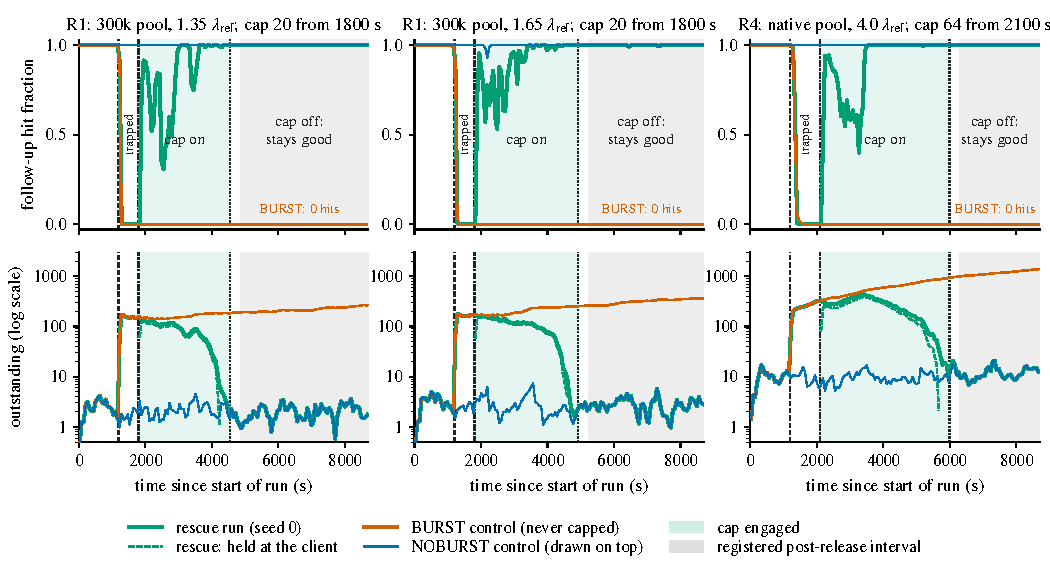
\includegraphics[width=\textwidth]{figs/fig_rescue.pdf}
\caption{Trap, rescue, release and persistence: the registered rescue tests R1 and R4, seed 0 of each cell. Each rescue run
(green) replays the arrival plan of a paired test's BURST run until a client-side session cap is engaged at $t_{\mathrm{on}}$
(dash-dotted; 1800\,s for R1 on the 300k pool, cap 20; 2100\,s for R4 with the native pool, cap 64); the cap is removed at
$t_{\mathrm{rel}}$ (dotted) once both client queues have been empty for 300\,s. The same-seed BURST (vermillion) and NOBURST (blue)
runs share its arrivals. Dashed: the burst of 200 sessions at 1200\,s. Top: follow-up hit fraction in 60\,s bins. Bottom:
outstanding work, requests in the engine plus sessions held at the client (log scale); dashed green: sessions held at the
client. Seeds 1 and 2 behave alike (Table~\ref{tab:rescue}).}\label{fig:rescue}
\end{figure*}

Corollary~\ref{cor:trapthr} leaves two ways out of a trap. One is to \emph{starve} it: bring the arrival rate below $\lmiss$
until the busy period ends. The other is to leave model~F: make turns hit again, which requires the sessions that compete for
the pool to fall below the onset $n_b$, without lowering the offered load. A client-side session cap does this.

\paragraph{Starving the trap: refusing arrivals sheds sessions, and is slow.} The corollary says how far and how long: below $\lmiss$, not below the
trapped throughput $D(\lambda)$, and for $V_{\mathrm{tot}}/(1-\lambda'/\lmiss)$, which diverges as $\lambda'\uparrow\lmiss$. In
the all-miss fluid at 1.65~$\lref$ (300k), a cut to $1.18\lmiss$, below $D=1.22\lmiss$, makes the backlog dip by 0.3\% and grow
again, and a cut to $0.9\lmiss$ drains it only after about 15 hours (Appendix~\ref{app:trap}). The registered SHED test at
1.35~$\lref$ on the 300k pool stopped arrivals entirely from 1800\,s, 600\,s after a burst. A 600\,s stop refused 56--59 sessions
and left both runs stuck; a 3600\,s stop refused 355--378 and left both good (\S\ref{sec:validation}). Lu et al.\ show in
simulation that lowering post-surge arrivals reverses the outcome, and observe that the throughput measured in the collapsed state
sets the scale of the cut~\citep{lu2026cachetrap}. Corollary~\ref{cor:trapthr}, proved in model~F, our idealization of an FCFS engine on which
every turn misses, sharpens this: there the cut must go below $\lmiss$, which lies below the trapped throughput $D(\lambda)$. Their
GPU-only simulations point the same way: the trap persisted at a cut to 0.2 of their reference rate (12 sessions/min) while the
trapped departures they measured were 0.20--0.31 of it. Their
systems keep some reuse in the trap, though, and with a host tier one seed in three recovered at cuts above the trapped departures
they measured, so the corollary does not describe them. The CUT test probes the corollary's setting on our engine (\S\ref{sec:validation}): a cut to below the trapped throughput of
the same seeds' uncut runs, and below the completion rate seen just before it, but above $\lmiss$, left all three CUT-A traps in
place to the end of the run, and a cut to 0.85~$\lref$, below $\lmiss$, shrank the CUT-B backlogs only slowly: all three were still
stuck at 8700\,s, where a drain at the uncut trapped throughput or at the completion rate seen before the cut would have reached the
onset by 4900--7600\,s. Each arm's registered rule rejected the naive reading; what singles out model~F against intermediate
readings is post hoc: CUT-A's late-window slopes and CUT-B's completions below the all-miss capacity.

\paragraph{Restoring reuse with a session cap.} A FIFO gate that admits at most $\ncap$ sessions, each holding its slot until its
last turn ends, makes the admitted sessions a closed system of $\min(n,\ncap)$ sessions (Proposition~\ref{prop:cap}). In the
quasi-static model the gate then empties if and only if $n_1<\ncap<n_2$, the stable and unstable fixed points of $\dot n=\lambda-\mu(n)$, and once it
is empty and removed the population stays in the good state's basin (Corollary~\ref{cor:rescue}). In model-F terms the cap keeps
the admitted sessions below the onset, so their turns hit again, and the excess waits at the client instead of in the engine's
queue, where every turn would miss. The registered rescue tests R1 (300k pool, cap 20, engaged at 1800\,s, 600\,s after the burst,
at 1.35 and 1.65~$\lref$) and R4 (native pool, cap 64, at 2100\,s, at 4.0~$\lref$) engaged the registered CAPPED caps inside
established traps: follow-up hit fraction 0.000--0.002 over the preceding 300\,s, with 139--324 requests or sessions outstanding.
All 9 runs were rescued without shedding a session (Table~\ref{tab:rescue}, Fig.~\ref{fig:rescue}). Hits returned within three
minutes, the backlog drained, and the cap was released at 3980--6140\,s, once the client queues had been empty for 300\,s. With
the cap removed, every run stayed good at the same arrival process for the remaining 2560--4720\,s, matching its NOBURST control in
follow-up hit fraction, outstanding work and turn latency, while the same-seed uncapped BURST run stayed at zero hits. The price is
waiting at the client: 386--569\,s per paused session on average, 38--78 (300k) and 222--230 (native) session-hours per run. In Lu
et al.'s SLO goodput (slowdown at most 4; we cannot apply their per-token latency condition), the burst cost the uncapped runs
99.2--100\% of the goodput of base sessions arriving in the following hour, against the same-seed NOBURST run, in all 30 registered
BURST runs (in 26 of them no such session met the slowdown target, so there the loss is 100\% under either definition); the rescue
cost 45--97\% in that hour, depending on the reference latency, but restored the evaluation window's goodput to within 1\% of
NOBURST (Appendix~\ref{app:dataonly}).

\begin{table}[t]
\centering\footnotesize
\caption{The registered rescue tests R1 and R4 (seeds 0, 1, 2); ranges over seeds. After release: follow-up hit fraction and mean
outstanding work over $[t_{\mathrm{rel}}+300,\,8700)$\,s for the rescue run and, over the same interval, its same-seed controls.
Delay: session-hours of pauses and admission waits at the client. Rows below the release time are descriptive, computed after the
registered verdict.}\label{tab:rescue}
\setlength{\tabcolsep}{3pt}
\begin{tabular}{@{}>{\raggedright\arraybackslash}p{2.3cm} c c c@{}}
\toprule
 & R1, 300k & R1, 300k & R4, native\\
 & 1.35 $\lref$ & 1.65 $\lref$ & 4.0 $\lref$\\
\midrule
cap; engaged at & 20; 1800\,s & 20; 1800\,s & 64; 2100\,s\\
rescued (relapses) & 3/3 (0) & 3/3 (0) & 3/3 (0)\\
release $t_{\mathrm{rel}}$ (s) & 3980--4550 & 4430--4920 & 5980--6140\\
\addlinespace
\multicolumn{4}{@{}l}{\emph{after release: follow-up hit fraction}}\\
\quad rescue & 0.999--1.000 & 0.994--1.000 & 1.000\\
\quad NOBURST & 0.999--1.000 & 0.991--1.000 & 1.000\\
\quad BURST & 0.000 & 0.000 & 0.000\\
\multicolumn{4}{@{}l}{\emph{after release: mean outstanding work}}\\
\quad rescue & 1.9--2.2 & 2.5--2.8 & 8.8--11.8\\
\quad NOBURST & 1.9--2.2 & 2.5--3.1 & 8.8--11.8\\
\quad BURST & 195--219 & 272--317 & 1133--1178\\
\addlinespace
sessions paused & 121--130 & 138--143 & 220--251\\
delay (session-h) & 38--65 & 50--78 & 222--230\\
\bottomrule
\end{tabular}
\end{table}

\paragraph{What the rescue does and does not show.} Persistence here means that the drained state sustains itself once the cap no
longer binds: the release rule waits until the gate is empty, so the tests do not cover a release while the cap still binds, and
the cap is engaged at a fixed time, not on an online signal. The frozen first-principles model predicted the rescue in every cell,
but 4 of its 9 release times fell outside its $\pm15$\% tolerance (R4 released 19--22\% late; Appendix~\ref{app:frozen}). Lu et
al.\ restore service on hardware by terminating the burst sessions at the end of the burst, when the trap is incipient, prevent it
with their controller active before the surge, rescue an established trap in simulation by activating their controller late (and
leaving it on), and report one hardware run in which CONCUR's hit rate fell
to 0.33 before its concurrency window contracted and recovered slowly, with the controller left on and no release
test~\citep{lu2026cachetrap}. What our tests add is a registered, replicated rescue of an \emph{established} zero-hit trap at the same
offered load, without shedding, with release of the control and persistence of the good state after it.
